Recall the general DAE representation:
\begin{equation}
E\dot{x} = Ax + Bu + Fw + g
\end{equation}Introducing the ODE representation that also can be extracted:
\begin{equation}
\dot{x} = Ax + Bu + g
\end{equation}
\begin{equation}
w  = Hx + Mu + q
\end{equation} Here it might be tempting to create the SFGs from the ODE instead, since one can extract the SFGs  for the states and algebraic variables separately. But notice, now the states does not depend at all on the algebraic variables in w. This is still a correct system, since algebraic variables is only a combination of states,other algebraic variables and constants thus can be reduced and replaced by other states and a constant. But even though it is mathematically correct, we have lost information. The causality is broken, and a user that has declared states that depends on algebraic variables can no longer view and analyse such relations inside ProMoVis. If we consider the fictional, system:

\begin{equation}
\dot{x_1}=x_2+w_1+u_2
\end{equation}
\begin{equation}
\dot{x_2}=x_3+u_1
\end{equation}
\begin{equation}
\dot{x_3}=x_1
\end{equation}
\begin{equation}
w_1=x_3+x_2
\end{equation}The DAE representation of the system is then:
\begin{equation}
\begin{bmatrix}  1 & 0 & 0 \\ 0 & 1 & 0  \\ 0 & 0 & 1 \\ 0 & 0 & 0   \end{bmatrix}  \left[ \begin{array}{c} \dot{x_1} \\ \dot{x_2} \\ \dot{x_3} \end{array} \right]
= \begin{bmatrix} 0 & 1 & 0 \\ 0 & 0 & 1 \\ 1 & 0 & 0 \\ 0 & 1 & 1 \end{bmatrix}  \left[ \begin{array}{c} x_1 \\ x_2 \\ x_3 \end{array} \right] + \begin{bmatrix} 0 & 1 \\ 1 & 0 \\ 0 & 0 \\ 0 & 0 \end{bmatrix} \left[ \begin{array}{c} u_1 \\ u_2 \end{array} \right]+
\begin{bmatrix} 1 \\ 0 \\ 0  \\ -1 \end{bmatrix} \left[ \begin{array}{c} w_1 \end{array} \right]
\label{fig:eqDAE}
\end{equation}
%
\begin{figure}
\fbox{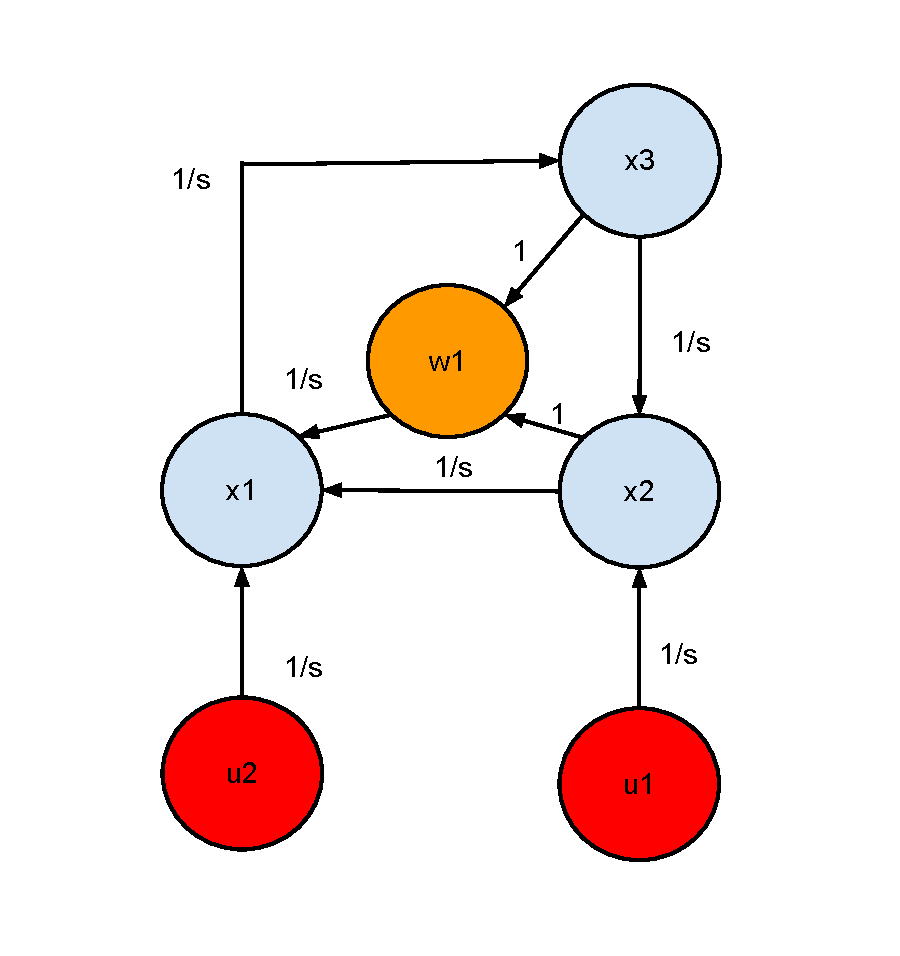
\includegraphics[scale=0.3,bb=0 0 153mm 162mm] {Figures/DAESFG.pdf}} 
\caption{SFG corresponding to the DAE in EQ. ~\ref{fig:eqDAE}.}
\label{fig:sfgDAE}
\end{figure}
%
The ODE-representation of the same system would become:
\begin{equation}\left[ \begin{array}{c} \dot{x_1} \\ \dot{x_2} \\ \dot{x_3} \end{array} \right]
= \begin{bmatrix} 0 & 2 & 1 \\ 0 & 0 & 1 \\ 1 & 0 & 0 \end{bmatrix} \left[ \begin{array}{c} x_1 \\ x_2 \\ x_3 \end{array} \right] + \begin{bmatrix} 0 & 1 \\ 1 & 0 \\ 0 & 0 \end{bmatrix}  \left[ \begin{array}{c} u_1 \\ u_2 \end{array} \right]
\label{fig:eqODEett}
\end{equation}
\begin{equation}\left[ \begin{array}{c} w_1  \end{array} \right]
=  \begin{bmatrix} 0 & 1 & 1\end{bmatrix} \left[ \begin{array}{c} x_1 \\ x_2 \\ x_3 \end{array} \right] + \begin{bmatrix} 0 & 0 \end{bmatrix}  \left[ \begin{array}{c} u_1 \\ u_2 \end{array} \right]
\label{fig:eqODE}
\end{equation}
\begin{figure}
\fbox{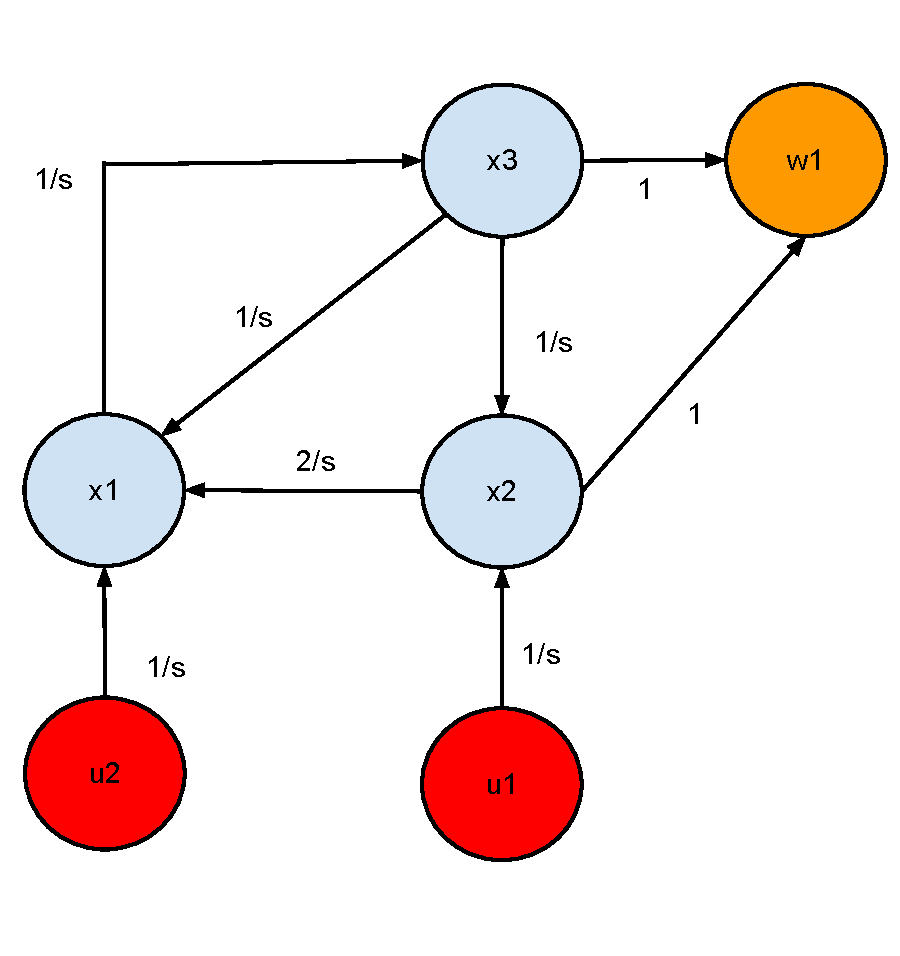
\includegraphics[scale=0.3,bb=0 0 153mm 162mm] {Figures/ODESFG.pdf}}
\caption{SFG corresponding to the ODE in EQ. ~\ref{fig:eqODEett} and EQ. ~\ref{fig:eqODE}.}
\label{fig:sfgODE}
\end{figure}%
As we can see, when comparing the SFG's in Fig. \ref{fig:sfgDAE} and Fig. \ref{fig:sfgODE}, the SFG-representations of the two systems will differ, we no longer can see the relation between $x_1$ and $w_1$. This is a problem since a user might want to analyse the relation between the algebraic variable and other points in the system directly.

